\subsection{Opto Switch Driver Module (OD)}

The Opto Switch Driver Module (OD) is an interface between module \mu M and the Opto Switch Module (OS).

\subsubsection*{Requirements}

Experiments have shown that at least \SI{50}{\mA} are required to obtain  clearly separated
voltage levels at the output of OS (.Prx).

\subsubsection*{Implementation}


\begin{figure}[h]
    \centering
    \includegraphics[width=0.8\textwidth]{MA/OD/OD}
    \caption{OD - schematic, based on datasheet \cite{noauthor_sn74lvc2g17_2002}}
\end{figure}

\begin{table}[H]
    \centering
    \begin{threeparttable}[b]
        \begin{tabularx}{\linewidth}{ >
                    {\hsize=.25\hsize}X >
                    {\hsize=0.5\hsize}X >
                    {\hsize=.25\hsize}X  >
                    {\hsize=.5\hsize}X >
                    {\hsize=.25\hsize}X  >
                    {\hsize=3\hsize}X
            }
                  & \multicolumn{4}{c}{Pin mapping} &                                                                             \\
            \cmidrule(lr){3-6}
            Id    & Net                             & Nb. & Name         & Type            & Function                             \\
            \midrule
            $U_1$ & .EOD                            & 1   & \texttt{1A}  & \leftharpoonup  & buffer input controlled by \mu C     \\
            $U_1$ & .EOD                            & 3   & \texttt{2A}  & \leftharpoonup  & buffer input controlled by \mu C     \\
            $U_1$ & \Gnd                            & 2   & \texttt{GND} & \Gnd            &                                      \\
            $U_1$ & Y                               & 4   & \texttt{1Y}  & \rightharpoonup & buffer output                        \\
            $U_1$ & .3V3                            & 5   & \texttt{VCC} & \leftarrow      & power supply                         \\
            $U_1$ & Y                               & 6   & \texttt{2Y}  & \rightharpoonup & buffer output                        \\
            $R_c$ & Y                               & 1   & \texttt{1}   &                 &                                      \\
            $R_c$ & .V\textsubscript{OS}            & 2   & \texttt{2}   &                 & anode voltage of photodiode          \\
            $R_p$ & .3V3                            & 1   & \texttt{1}   &                 & upper rail for pullup resistor       \\
            $R_p$ & .Prx                            & 2   & \texttt{2}   &                 & collector voltage of phototransistor \\
        \end{tabularx}
        \begin{tablenotes}
            \item []
        \end{tablenotes}
    \end{threeparttable}

\end{table}
\begin{table}[H]
    \centering
    \begin{threeparttable}[b]
        \begin{tabularx}{\linewidth}{ >{\hsize=.15\hsize}X >{\hsize=1.35\hsize}X >{\hsize=1.5\hsize}X }

            Id & Issue             & Potential solution      \\
            \midrule
            1  & power consumption & current source\tnote{1} \\
        \end{tabularx}
        \begin{tablenotes}
            \item [1] The current implementation is not ideal. It would be better to use a (programmable) current source to avoid burning power in the current
            limiting resistor. In addition, the optimum output current remains to be determined.
        \end{tablenotes}
    \end{threeparttable}
    \caption{OD - issues}
\end{table}
\clearpage
\begin{table}[H]
    \centering
    \begin{threeparttable}[b]
        \begin{tabularx}{\linewidth}{ >{\hsize=0.25\hsize}X >{\hsize=0.75\hsize}X >{\hsize=1.25\hsize}X >{\hsize=0.5\hsize}X >{\hsize=2.25\hsize}X}

            Id    & Desc                             & Order Code          & FF     & Rationale                                   \\
            \midrule
            $U_1$ & \cite{noauthor_sn74lvc2g17_2002} & SN74LVC2G17DCKR/473 & SC70/6 & high output power, parallel output\tnote{1} \\
            $R_p$ & \SI{1}{\kilo\ohm}                & generic             & 0603   & pull-up resistor\tnote{2}                   \\
            $R_c$ & \SI{20}{\ohm}                    & generic             & 0603   & current limit resistor \tnote{3}            \\
            $C_b$ & \SI{100}{\nF}, \SI{16}{\V}       & generic             & 0402   & bypass cap                                  \\
        \end{tabularx}
        \begin{tablenotes}
            \item [1] for a total rated maximum of \SI{48}{\milli\ampere}, low power consumption,
            the Smitt-Trigger inputs are not really necessary for this application.
            \item [2] We should explain why we choose this value. But as mentioned in Issue 1, we are likely
            to replace the current limit resistor with a current source in the near future.
            \item [3] idem
        \end{tablenotes}
    \end{threeparttable}
    \caption{OD - BOM}
    \label{table:wd1}
\end{table}









